\documentclass[8pt]{beamer}
\usepackage[utf8]{inputenc}
\usepackage{xcolor}
\usepackage{colortbl}
\usepackage{epsfig}
% \usepackage{cancel}
\usepackage{ulem}
% \usepackage{threeparttable} % Joao Pela: 
\usepackage{amsmath}
\usepackage{hyperref}
\usepackage{siunitx}  % Allows easy x10^ for numbers
\usepackage{appendixnumberbeamer}

\usetheme{Madrid}

\author[J. Pela]{João Pela}
\title{QCD VBFMET samples MadGraph Studies}
\institute[ICL]{Imperial College London}
\date{2015-08-04}

% The log drawn in the upper right corner.
\logo{\includegraphics[height=0.115\paperheight]{img/Logo_CMSICL.png}}

\begin{document}
\setlength{\unitlength}{1mm}

% ###################################################
\begin{frame}
  \titlepage
\end{frame}

% ###################################################
\begin{frame}{Introduction}

\begin{block}{Summary of PPD meeting}
  
\begin{itemize}
  \item Presentation was made on our proposal for QCD VBF-MET samples and feedback was requested.
  \item Main concern points were:
  \begin{itemize}
    \item The huge amount of time required by obtaining events in the low pT hats (filter efficiency is  $5 \times 10^{-6}$ for working point A at lowest pT hat) 
    \item The amount of events going over DIGI (apparently this request would be $\sim15\%$ of the a last campaign)
  \end{itemize}
  \item The size of the sample itself did not sound like a big problem.
  \item It was suggested to look into looking into MadGraph with some reasonable generator cuts in order to reduce filtering needs and processing time. 
\end{itemize}

\end{block}

\begin{block}{Steps to preform}

After the meeting in a chat within our group it was suggested 

\begin{itemize}
  \item Looking into usable MadGraph variables, avoid $\Delta\phi$ or even $\Delta\eta$ cuts.
  \item Study the relationship between generator partons and generator jets
  \item Study filter efficiency
  \item (I would also like to) Look into parton versus HLT objects
  \item (I would also like to) Look into a mini sample of this versus data. 
\end{itemize}

\end{block}

\end{frame}

% ###################################################
\begin{frame}{Introduction}

The event production runs on MadGraph are controlled by a set of ``card'' files which contain all the parameters that are relevant. For the \textit{run\_card.dat} here are the relevant parameters for our analysis.

\begin{block}{Relevant run\_card.dat parameters}

\begin{itemize}
  \item \textbf{nevents}: Number of unweighted events requested 
  \item \textbf{ptj}: (default 20) minimum pt for the jets 
  \item \textbf{etaj}: (default 5.0) max rap for the jets 
  \item \textbf{drjj}: (default 0.4) min distance between jets
  \item \textbf{mmjj}: (default 0.0) min invariant mass of a jet pair 
  \item \textbf{ptj1min}: (default 0.0) minimum pt for the leading jet in pt
  \item \textbf{ptj2min}: (default 0.0) minimum pt for the second jet in pt
  \item \textbf{deltaeta}: (default 0.0) minimum rapidity for two jets in the WBF case 
\end{itemize}

\end{block}

\end{frame}

% ###################################################
\begin{frame}{MadGraph process cross sections}

I have tried several working points to check what would be the necessary number of events to produce.

\begin{block}{Madgraph working points}

\begin{table}[htp]
\centering

\resizebox{\linewidth}{!}{
\begin{tabular}{|c|c|c|c||c|l|}
\hline
etaj & ptj1min & ptj2min & mmjj & Cross Section [pb] & Notes \\ 
\hline
 5.0 &       0 &       0 &    0 & $\num{7.008e+08} \pm \num{6.648e+05}$ & MadGraph Default values \\
 4.8 &       0 &       0 &    0 & $\num{6.879e+08} \pm \num{6.644e+05}$ & Reduncing jet eta range \\
 4.8 &      40 &      40 &    0 & $\num{5.266e+07} \pm \num{4.772e+04}$ & Require 2 jets with $p_\perp>40$ GeV\\
\hline\hline
 4.8 &      40 &      40 &  800 & $\num{8.911e+05} \pm 653.2$           & Working Point A \\
\hline\hline
 4.8 &      35 &      35 &  800 & $\num{1.21e+06}  \pm 878.9$           & WP A: dijet $p_\perp$ -5 GeV \\
 4.8 &      30 &      30 &  800 & $\num{1.699e+06} \pm 1304$            & WP A: dijet $p_\perp$ -10 GeV \\
\hline\hline
 4.8 &      40 &      40 &  700 & $\num{1.234e+06} \pm 940$             & WP A: dijet $p_\perp$ -100 GeV \\
 4.8 &      40 &      40 &  900 & $\num{6.611e+05} \pm 482.6$           & WP A: dijet $p_\perp$ +100 GeV \\
 4.8 &      40 &      40 & 1000 & $\num{5.009e+05} \pm 377$             & WP A: dijet $p_\perp$ +200 GeV \\
\hline\hline
 4.8 &      50 &      50 & 1000 & $\num{2.948e+05} \pm 222.8$           & Working Point B \\
\hline
\end{tabular}
}

\end{table}


\end{block}

\tiny
\begin{itemize}
  \item Cross section obtained from generating 100k events with MG5\_aMC\_v2.3.0 (from 2015-07-01)
  \item Process \texttt{p p > j j} where \texttt{j = g u c d s u$\sim$ c$\sim$ d$\sim$ s$\sim$}
  \item Working Point A and be are basically the same as the previously proposed filters working points but without $\Delta\phi$ or $\Delta\eta$ 
\end{itemize}

The with pythia the total cross section of the pT hats to generate was: \num{1.87E+08} two orders of magnitude higher.

\end{frame}

% ###################################################
\begin{frame}{CMSSW and Pythia8 hadronization}
  
I have decided to proceed with Working Point A and with the help of Chayanit was able to interface CMSSW with the produced MadGraph events. 

\begin{block}{CMSSW details}
  
\begin{itemize}
  \item CMSSW\_7\_1\_18 version
  \item Hadronization done by Hadronizer\_TuneCUETP8M1\_13TeV\_MLM\_5f\_max4j\_LHE\_pythia8\_cff
  \item Generator jets are AK4 GenJetsNoNu
\end{itemize}

\end{block}

\begin{block}{Matching results}

\resizebox{\linewidth}{!}{
\begin{tabular}{|c|c|c|c|c|}
\hline
Events in & Events Pass & Event Eff [\%] & xsec before [pb]                      & xsec match [pb] \\
\hline\hline
100000    &       17077 & $17.1 \pm 0.1$ & $\num{8.911e+05} \pm \num{6.532e+02}$ & $\num{1.522e+05} \pm \num{1.066e+03}$ \\
\hline
\end{tabular}
}

\end{block}

\begin{block}{Questions}

\begin{itemize}
  \item Which file to use: events.lhe.gz or unweighted\_events.lhe.gz (results with the unweighted events).
  \item Is this matching efficiency ok? 
  \item What cross section to use? Pre or post matching?
\end{itemize}

\end{block}

\end{frame}

% ###################################################
\begin{frame}{Matching Partons with Generator jets}
  
\begin{block}{Parton selection}

\begin{itemize}
  \item For partons selecting status:
  \begin{itemize}
    \item 23 - outgoing
    \item 24 - outgoing, nonperturbatively kicked out in diffraction
  \end{itemize}
\end{itemize}

\end{block}

\begin{block}{Pairing Partons and Generator Jets}

\begin{itemize}
  \item Selecting all generator jets within $\Delta R < 0.4$ (this may need to be a big bigger)
  \item From those selecting the generator jet with the lowest $p_\perp$ to the parton as a match.
  \begin{itemize}
    \item This avoids picking up the wrong jet from just picking lowest $\Delta R$
  \end{itemize}
\end{itemize}

\end{block}

\begin{block}{Pairing Results for 10k events}
  
\begin{itemize}
  \item Pythia8 matched events events: 1712
  \item Found genJet for 2 parton: 1489 (87.0\%)
  \item Found genJet for 1 parton: 212 (12.4\%)
  \item Found genJet for 2 parton: 11 (0.6\%)
  \item Matched genJet was not the lowest $\Delta R$: 120
\end{itemize}

\end{block}

\end{frame}

% ###################################################
\begin{frame}{Parton vs Matched GenJet $p_\perp$}

\begin{block}
  
\begin{columns}

\column[t]{0.45\linewidth}
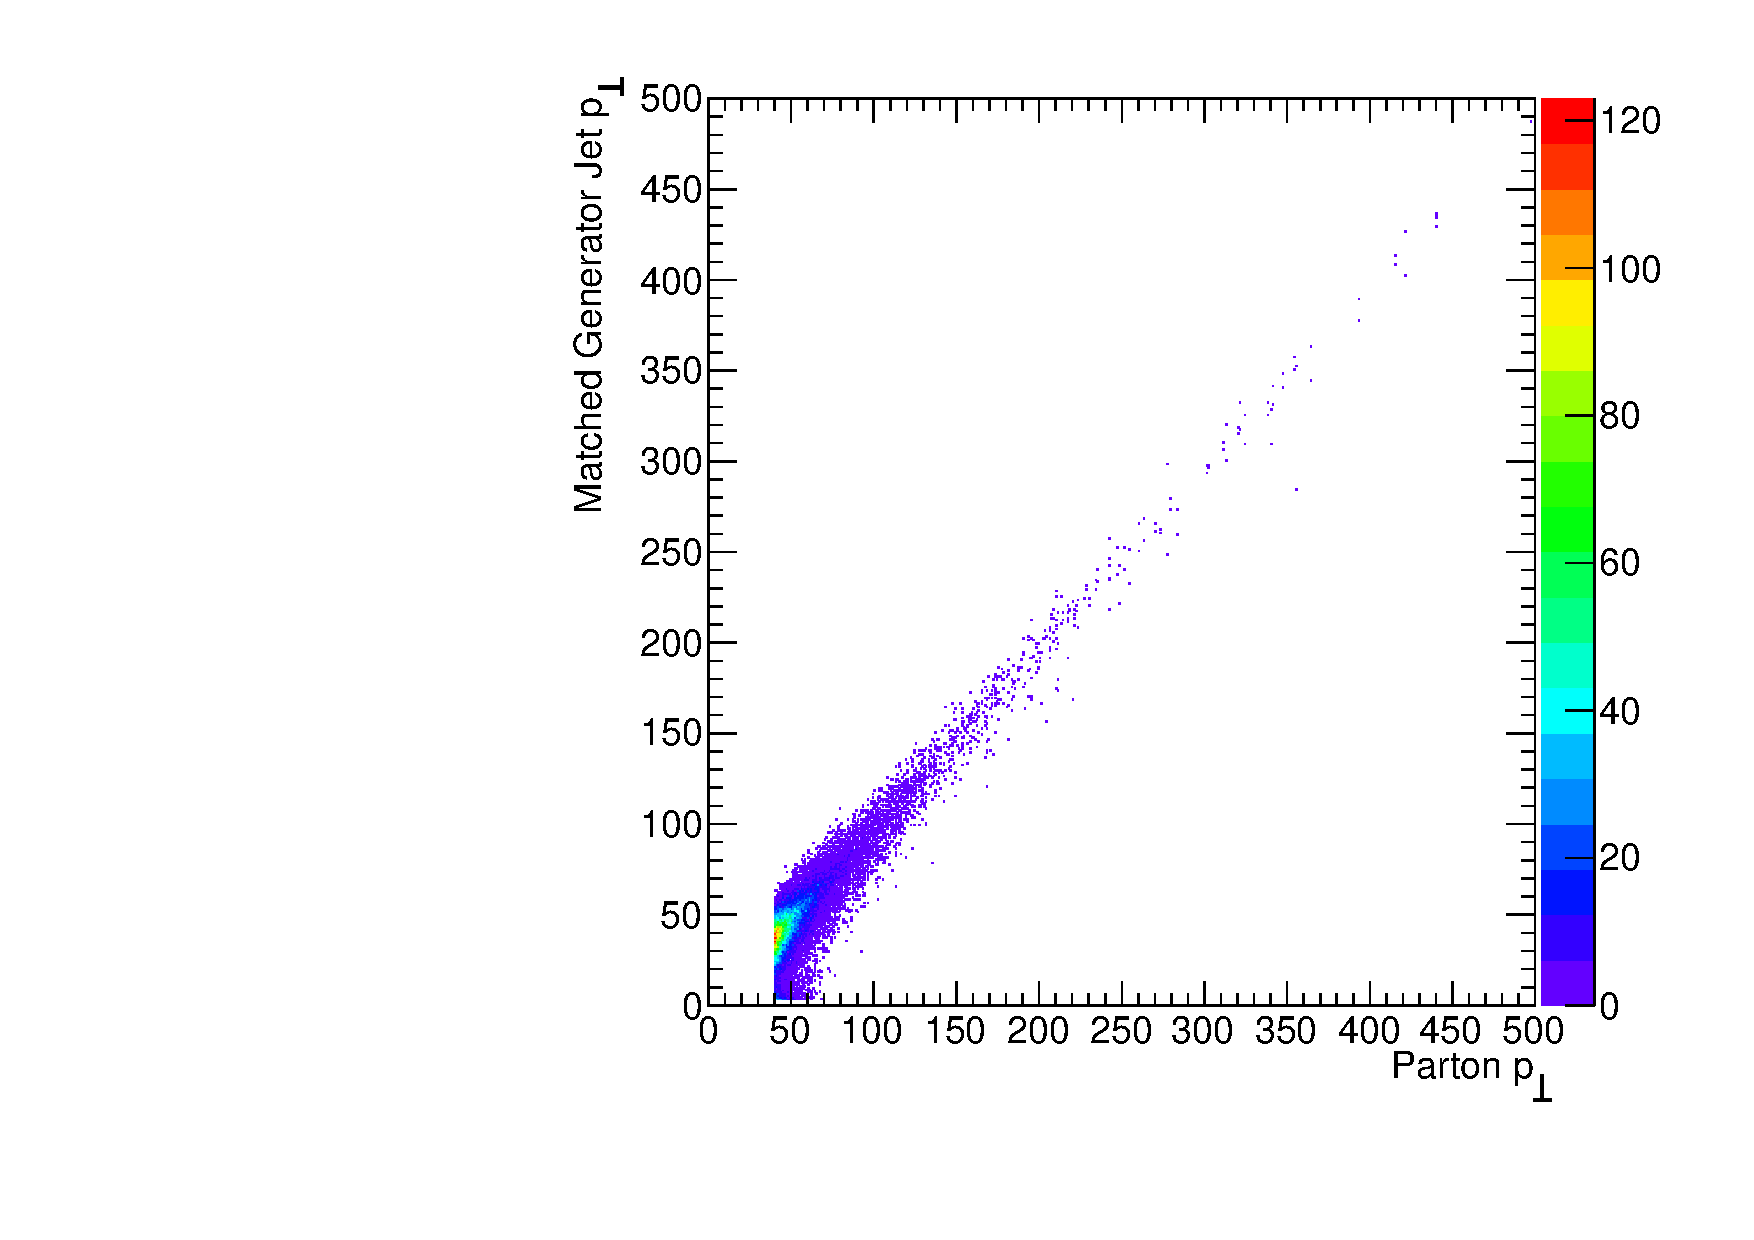
\includegraphics[width=\linewidth]{PartonvsGenJet_Pt.pdf}

\column[t]{0.45\linewidth}
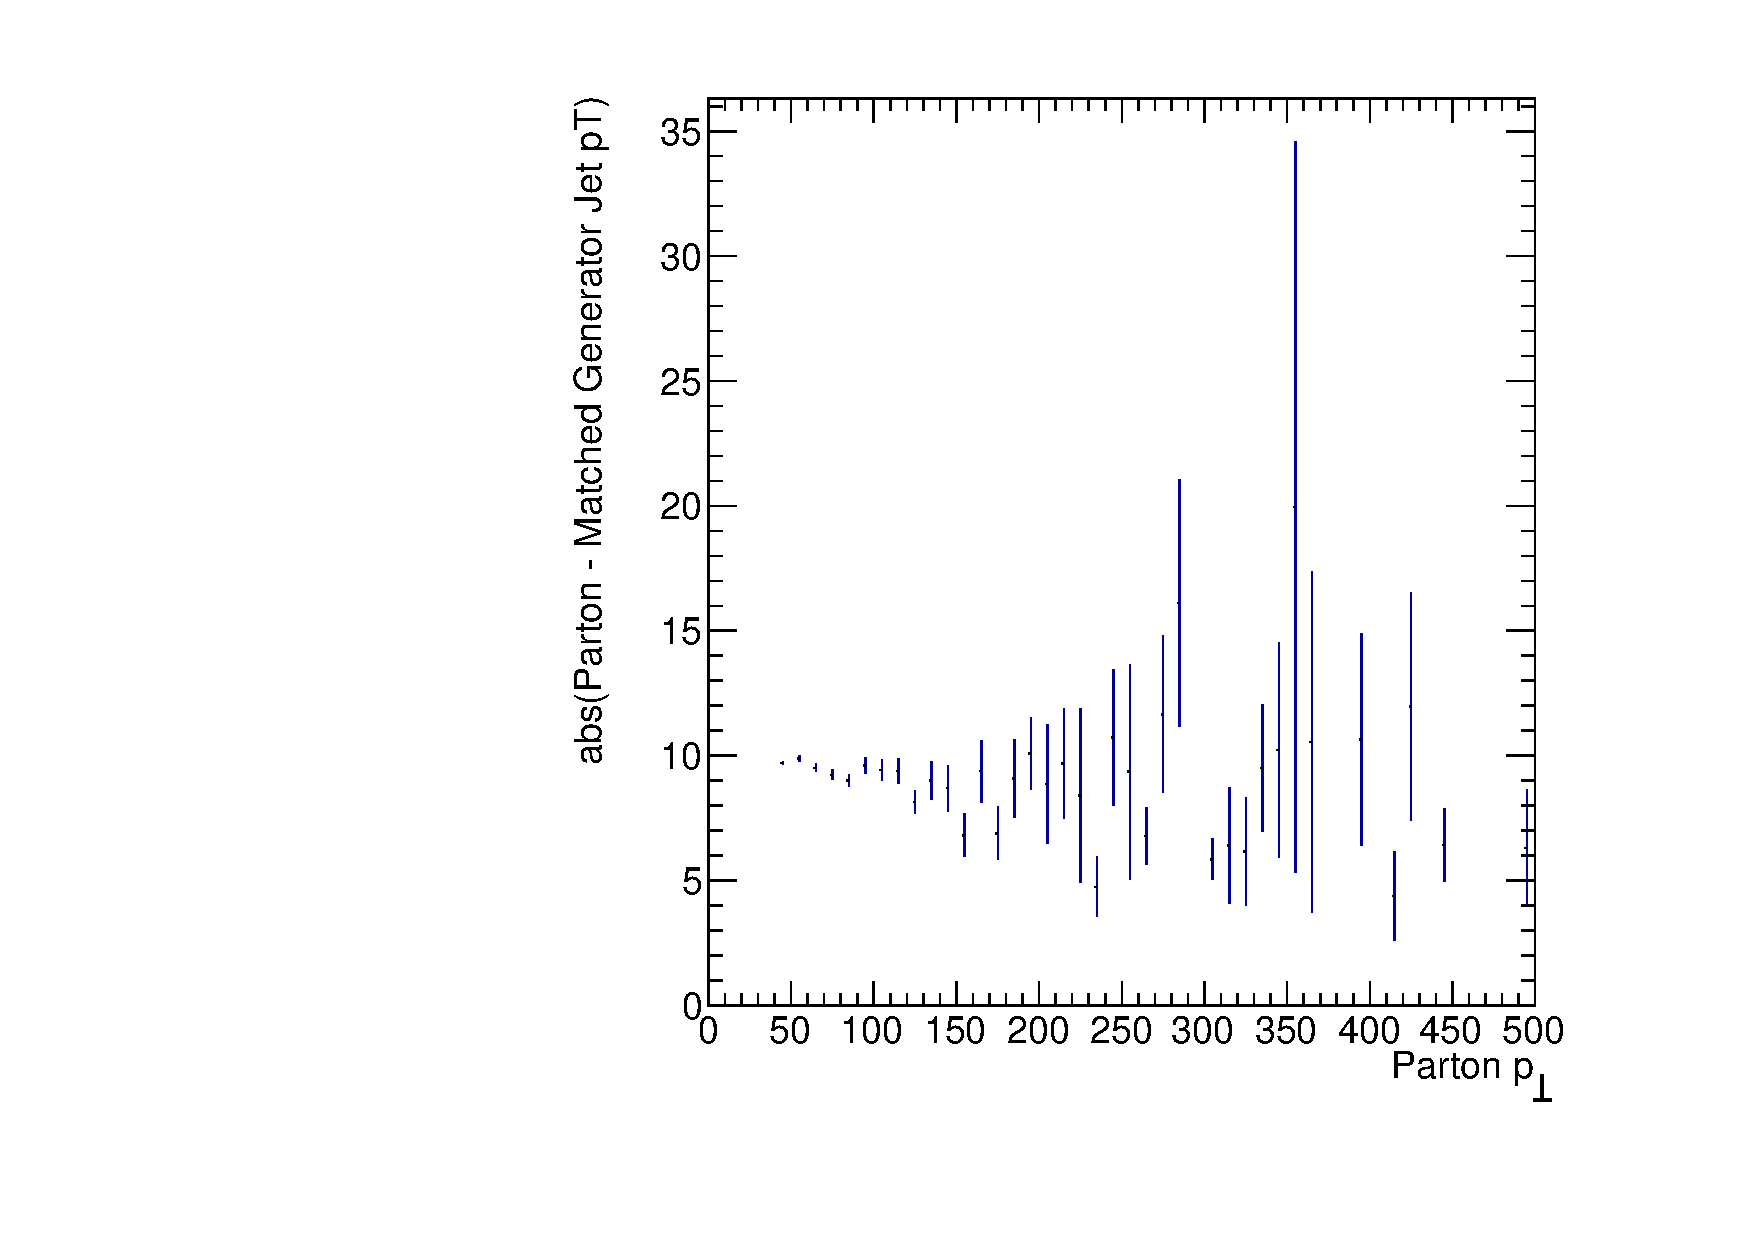
\includegraphics[width=\linewidth]{Profile_PartonvsGenJet_DiffPt.pdf}

\end{columns}

\end{block}

\end{frame}

% ###################################################
\begin{frame}{Parton vs Matched GenJet $\eta$}

\begin{block}

\begin{columns}

\column[t]{0.45\linewidth}
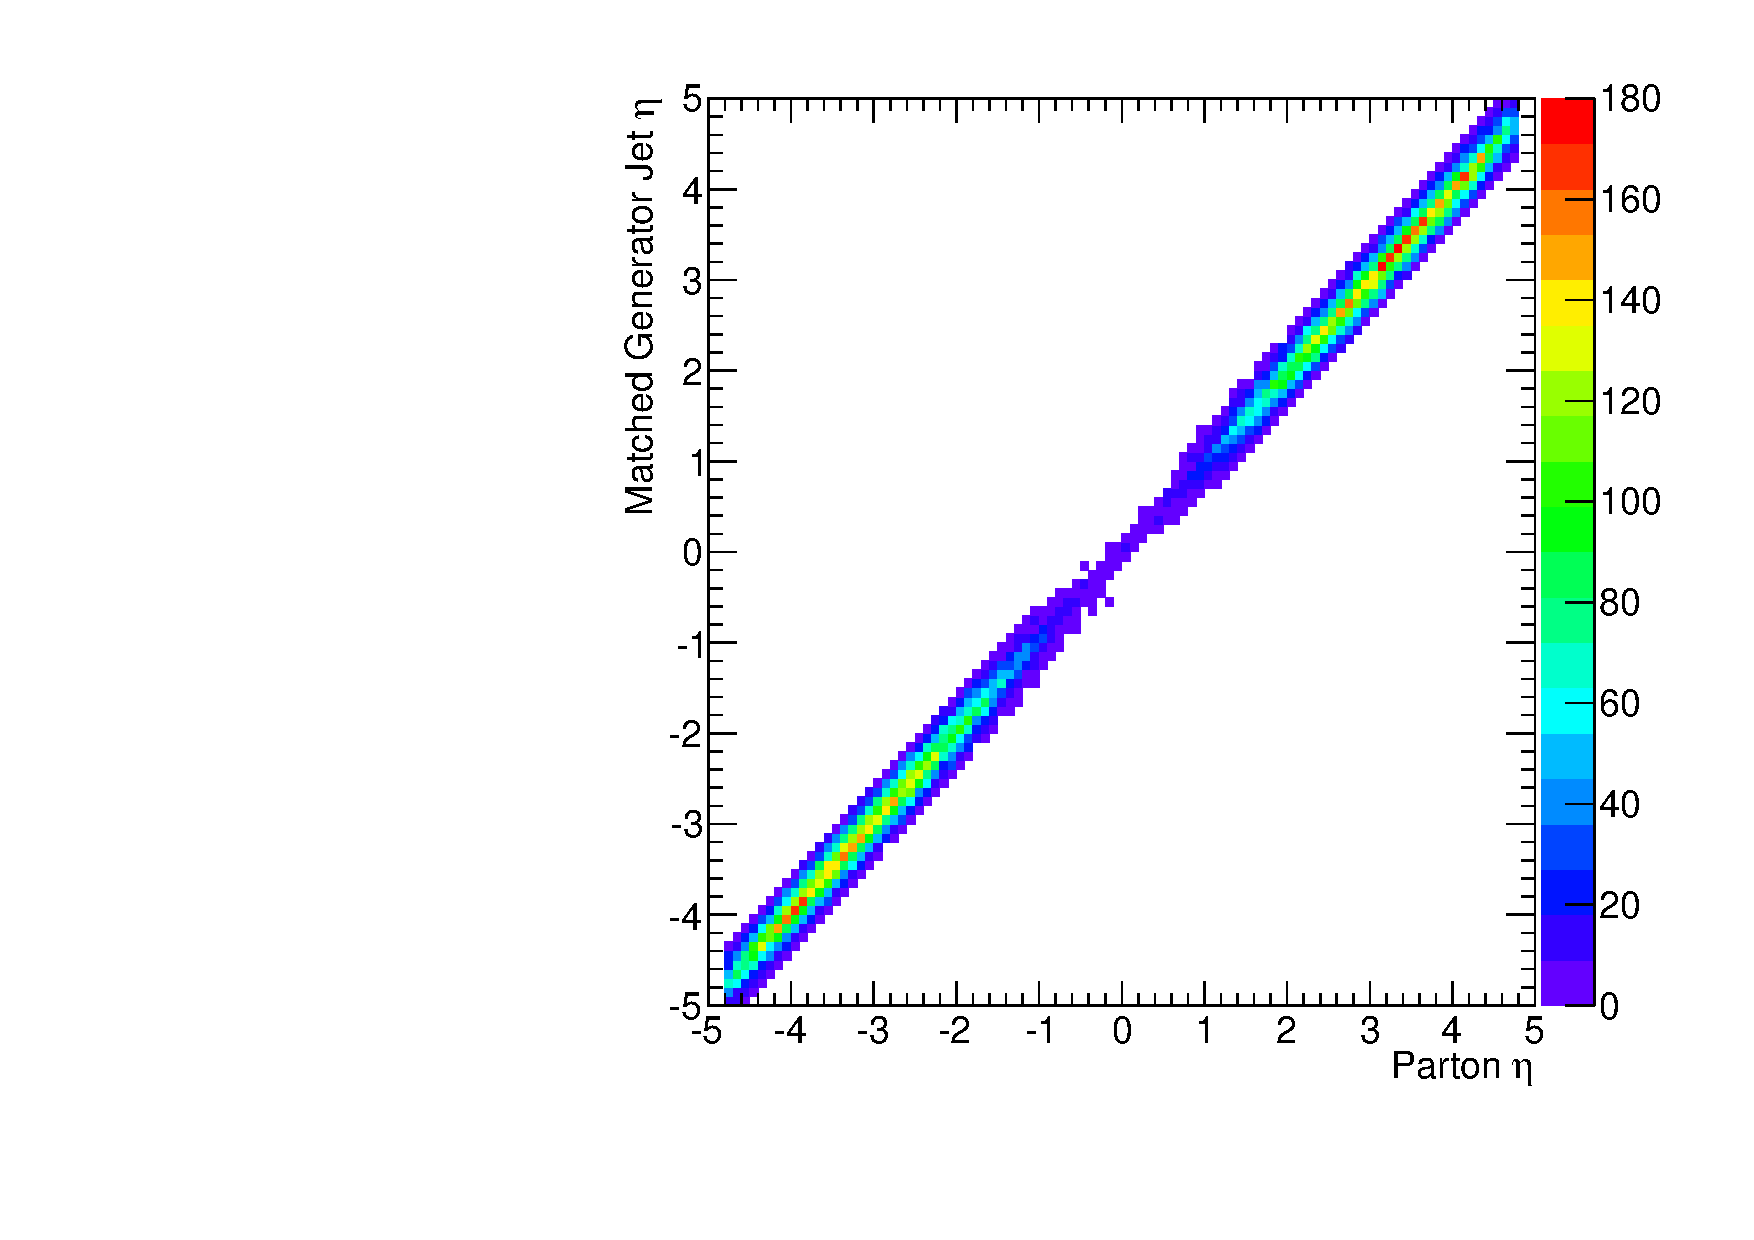
\includegraphics[width=\linewidth]{PartonvsGenJet_Eta.pdf}

\column[t]{0.45\linewidth}
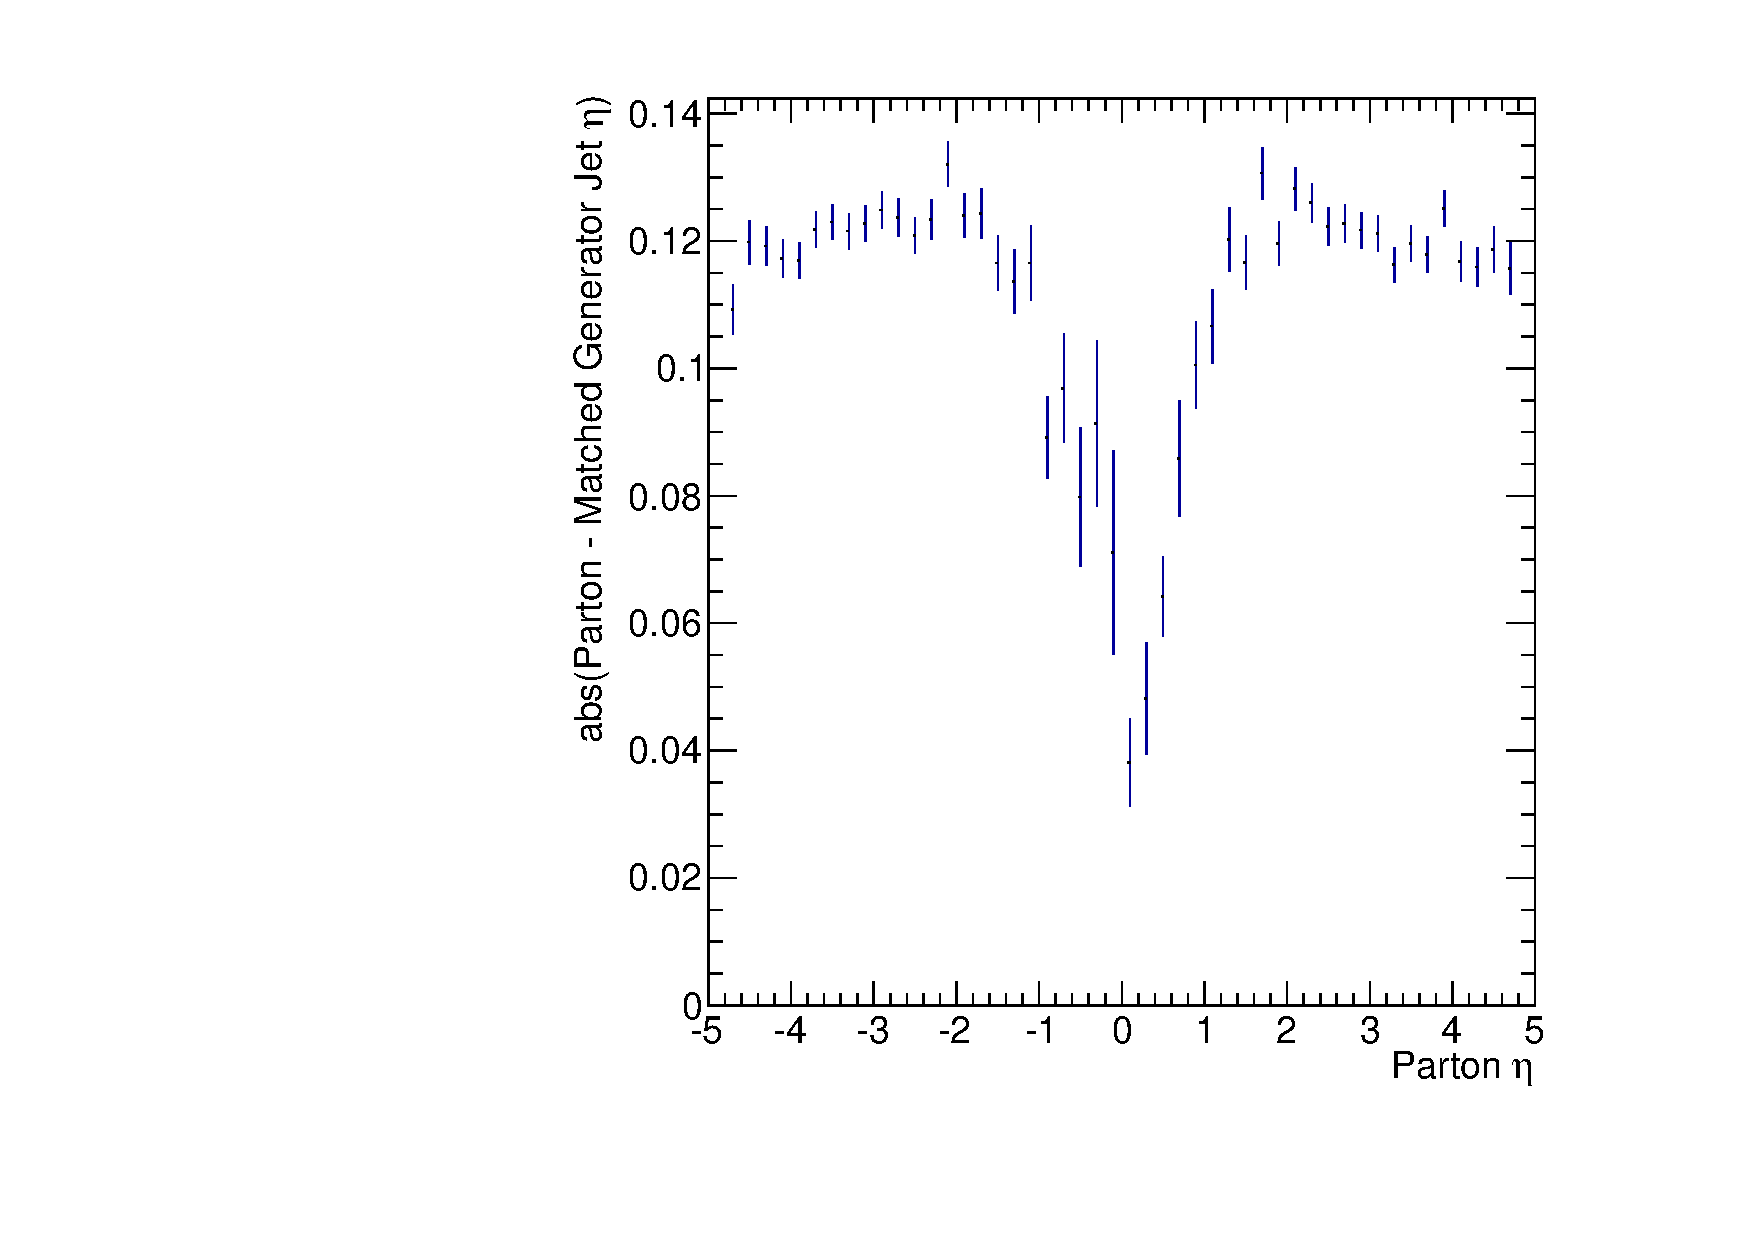
\includegraphics[width=\linewidth]{Profile_PartonvsGenJet_DiffEta.pdf}

\end{columns}

\end{block}

\end{frame}


\end{document}
